\chapter{Arquitetura}
\begin{figure}[H]
	\centering
		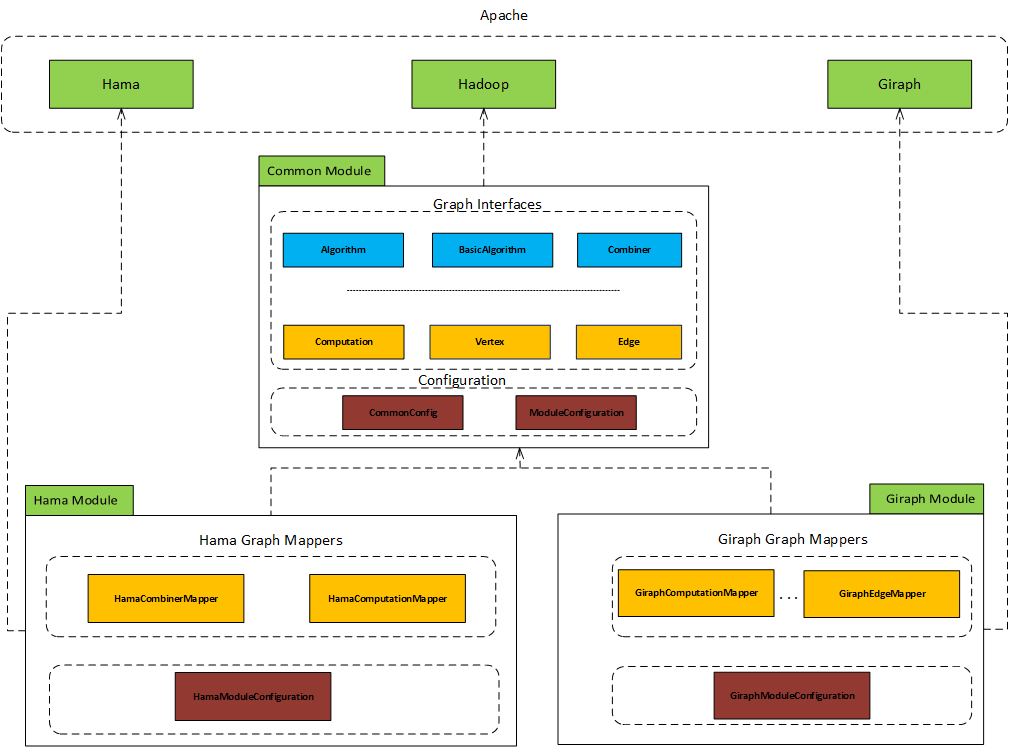
\includegraphics[width=\linewidth]{arquitetura}
	\caption{Em azul estão as interfaces e classes que devem ser 
	implementadas por um programador que esteja interessado em implementar 
um algoritmo no módulo comum. As outras cores representam interfaces e classes 
que devem ser implementadas para criar-se um novo módulo sobre o módulo comum.}
	\label{fig:arquitetura}
\end{figure}

Para que se torne possível a utilização das interfaces disponibilizadas pelo 
módulo comum existe a necessidade de realizar um conjunto de configurações. 
Devido a essa necessidade e para que essas 
configurações sejam feitas de forma independente da plataforma,
criou-se a interface \texttt{ModuleConfig} que será registada na classe \texttt{CommonConfig}.
Os módulos respetivos as plataformas que estão a mapear para o módulo comum necessitam implementar 
\texttt{ModuleConfig} e realizar as configurações necessárias para a respetiva 
plataforma. Esta implementação implica para que se use o módulo comum se proceda 
ao uso do \texttt{CommonConfig}.

O módulo comum foi construído de modo a que se possa fazer proveito das 
interfaces programáveis disponibilizas pelas plataformas Apache Giraph e Apache 
Hama. Usando o módulo comum é possível usar tipos de mensagens e tipos de valor 
para vértices diferentes, mesmo usando a plataforma Apache Hama onde isto não é 
possível. Igualmente, no Hama o tipo usado nos agregadores deve ser mesmo que o tipo
de valor dos vértices mas usando o módulo comum esta restrição é inexistente.

Contudo, nem todas as funcionalidades são disponibilizadas pelo módulo comum.
O \texttt{MasterCompute} não é disponibilizado devido a falta da sua implementação no Hama e dificuldade
de implementar-lo sem alterar diretamente o código da plataforma.
O \textit{input/output} é diferente nas 
duas plataformas daí que não exista nenhuma abstração no módulo comum.



\section{A plataforma}
A arquitetura da plataforma está dividida em duas partes, as classes que devem ser implementadas ou derivadas para que seja possível correr um algoritmo na plataforma e as classes que devem ser mapeadas para que seja possível adicionar um novo módulo à plataforma.

\subsubsection*{Novos módulos}

Assim, para que seja possível adicionar um novo módulo à plataforma é necessário o mapeamento dos tipos
\begin{itemize}
	\item Computation - Tendo a mesma função que o Computation do Giraph, e capacidade de dar informação geral sobre o grafo.
	\item Vertex - Representa um único vértice, dando a possibilidade de conhecer e alterar o estado deste.
	\item Edge - Representa uma única aresta e, como o vértice, possibilita conhecer e alterar o estado desta.
\end{itemize}
Foi feita uma divisão entre a lógica relacionada com o grafo e a relacionada com os vértices como aquela existente da plataforma Giraph pois isto possibilitaria a simplificação da lógica associada a estes.

\subsubsection*{Configuração}
A criação de um novo módulo também envolve o mapeamento das configurações necessários e para isso é necessário implementar a classe \texttt{ModuleConfiguration}.

Esta classe apresenta métodos que serão chamados quando forem usadas algumas componentes como agregadores ou combinadores e também métodos que servem para mapear as configurações mais comuns. 
Tem também um método extra que deve ser chamado por um programador que implemente um algoritmo onde são realizadas quaisquer configurações extras.

Assim, é de seguida apresentado um exemplo de configuração da plataforma.

\begin{verbatim}
		GiraphConfiguration conf = new GiraphConfiguration();

		// Configurações exclusivas à plataforma escolhida, como Input/Output, 
		// podem ser realizadas aqui
		
		//Para mudar a plataforma a ser usada bastaria mudar o ModuleConfiguration usado
		GiraphModuleConfiguration giraphConfig = new GiraphModuleConfiguration(conf);
		
		CommonConfig commonConfig = new CommonConfig(giraphConfig);
		
		// Configurações relacionadas com o algoritmo a correr
		commonConfig.setAlgorithmClass(ExampleAlgorithm.class);
		
		commonConfig.setCombinerClass(IntSumCombiner.class);
		
		commonConfig.registerAggregator("SumAgg", LongSumAggregator.class);
		commonConfig.registerAggregator("OrAgg", BooleanOrAggregator.class);
		
		// Precisa sempre de ser chamado para configurações finais
		commonConfig.preparePlatformConfig();
		
		// Pode agora ser chamado o método que leva ao início da computação
		// na plataforma especificada.
\end{verbatim}

\subsubsection*{Implementar algoritmos}
Um programador que esteja interessado em implementar um algoritmo nesta plataforma terá que derivar das classes \texttt{Algorithm} ou \texttt{BasicAlgorithm}.

A classe \texttt{Algorithm} dá acesso aos métodos de \texttt{Computation}, é onde está presente o método \texttt{compute} e onde deve ser implementado a lógica do algoritmo.

Apresenta quatro parâmetros genéricos que possibilitam decidir os tipos do identificador do vértice, do valor do vértice, do valor das arestas e da mensagem. Sendo que \texttt{BasicAlgorithm} é um \texttt{Algorithm} onde os tipos do valor do vértice e da mensagem são os mesmos.

A plataforma tem, também, as classes \texttt{Aggregator} e \texttt{Combiner} que representam agregadores e combinadores, respetivamente e dão a possibilidade ao programador que criar os seus próprios agregadores e combinadores, já existindo alguns implementados.


